\documentclass{article}

\usepackage{amsfonts}
\usepackage{amsmath}
\usepackage{amssymb}
\usepackage{amsthm}
\usepackage{caption}
\usepackage{color}
\usepackage{enumerate}
\usepackage{fancyhdr}
\usepackage[margin=1in]{geometry}
\usepackage{hyperref}
\usepackage{graphicx}
\usepackage{latexsym}
\usepackage{listings}
\usepackage{mathrsfs}
\usepackage{natbib}
\usepackage[nottoc]{tocbibind}
\usepackage{setspace}
\usepackage{tikz}
\usepackage{tkz-graph}
\usepackage{url}

\providecommand{\all}{\ \forall \ }
\providecommand{\bs}{\backslash}
\providecommand{\e}{\varepsilon}
\providecommand{\E}{\ \exists \ }
\providecommand{\lm}[2]{\lim_{#1 \rightarrow #2}}
\providecommand{\m}[1]{\mathbb{#1}}
\providecommand{\mc}[1]{\mathcal{#1}}
\providecommand{\nv}{{}^{-1}}
\providecommand{\ov}[1]{\overline{#1}}
\providecommand{\p}{\newpage}
\providecommand{\q}{$\quad$ \newline}
\providecommand{\rt}{\rightarrow}
\providecommand{\Rt}{\Rightarrow}
\providecommand{\vc}[1]{\boldsymbol{#1}}
\providecommand{\wh}[1]{\widehat{#1}}

%\renewcommand\bibname{References}

\fancyhead{}
\fancyfoot{}
\fancyhead[R]{\thepage}
\fancyhead[C]{Landau}

\hypersetup{
    colorlinks,
    citecolor=black,
    filecolor=black,
    linkcolor=black,
    urlcolor=blue
}

\definecolor{dkgreen}{rgb}{0,0.6,0}
\definecolor{gray}{rgb}{0.5,0.5,0.5}
\definecolor{mauve}{rgb}{0.58,0,0.82}

\lstset{ 
 % basicstyle=\tiny,
  language=C,                % the language of the code
  numbers=none,
  numberfirstline=false,
  numbersep=5pt,                  % how far the line-numbers are from the code
  backgroundcolor=\color{white},      % choose the background color. You must add \usepackage{color}
  showspaces=false,               % show spaces adding particular underscores
  showstringspaces=false,         % underline spaces within strings
  showtabs=false,                 % show tabs within strings adding particular underscores
  frame=lrb,                   % adds a frame around the code
  rulecolor=\color{black},        % if not set, the frame-color may be changed on line-breaks within not-black text 
  tabsize=2,                      % sets default tabsize to 2 spaces
  captionpos=t,                   % sets the caption-position 
  breaklines=true,                % sets automatic line breaking
  breakatwhitespace=false,        % sets if automatic breaks should only happen at whitespace
  %title=\lstname,                   % show the filename of files included with \lstinputlisting;
  keywordstyle=\color{blue},          % keyword style
  commentstyle=\color{gray},       % comment style
  stringstyle=\color{dkgreen},         % string literal style
  escapeinside={\%*}{*)},            % if you want to add LaTeX within your code
  morekeywords={*, ...},               % if you want to add more keywords to the set
  xleftmargin=0.053in, % left horizontal offset of caption box
  xrightmargin=-.03in % right horizontal offset of caption box
}

\DeclareCaptionFont{white}{\color{white}}
\DeclareCaptionFormat{listing}{\parbox{\textwidth}{\colorbox{gray}{\parbox{\textwidth}{#1#2#3}}}}
\captionsetup[lstlisting]{format = listing, labelfont = white, textfont = white}
 %For caption-free listings, comment out the 3 lines above
 \lstset{frame = single}


%%% TITLE AND DATE

\title{\vspace{4cm} \hrule  \vspace{0.4cm} \huge
Dynamic Ledger: a tutorial
\vspace{0.4cm} \hrule}
\date{\today}


%%% DOCUMENT

\begin{document}
\begin{titlepage}

\maketitle

\begin{center}
\vspace{1cm}
\Large
\begin{center}
Will Landau \\ $\quad$ \\
Department of Statistics \\
Iowa State University \\ $\quad$ \\
\end{center}

\vfill
\large
Copyright \copyright ~Will Landau 2013. 
\end{center}
\end{titlepage}

\newpage 
\pagestyle{fancy}
\setcounter{page}{1}
\pagenumbering{roman}
\tableofcontents 

\newpage
\setcounter{page}{1}
\pagenumbering{arabic}
%\fancyhead[C]{\thesection}

\begin{flushleft}

\section{Introduction and basic usage}

\paragraph{} Dynamic Ledger is a standalone C program for managing personal finances. Unlike most other accounting software, it takes into account transaction delays and multiple credit accounts when it computes summaries. It also allows the user to easily condense the ledger periodically so that the file remains lightweight over time.

\paragraph{} According to the program's conceptual model, transactions flow through credit accounts and eventually arrive in partitions of bank accounts (i.e., Food, Bills, Medical, etc.). \q

\begin{center}
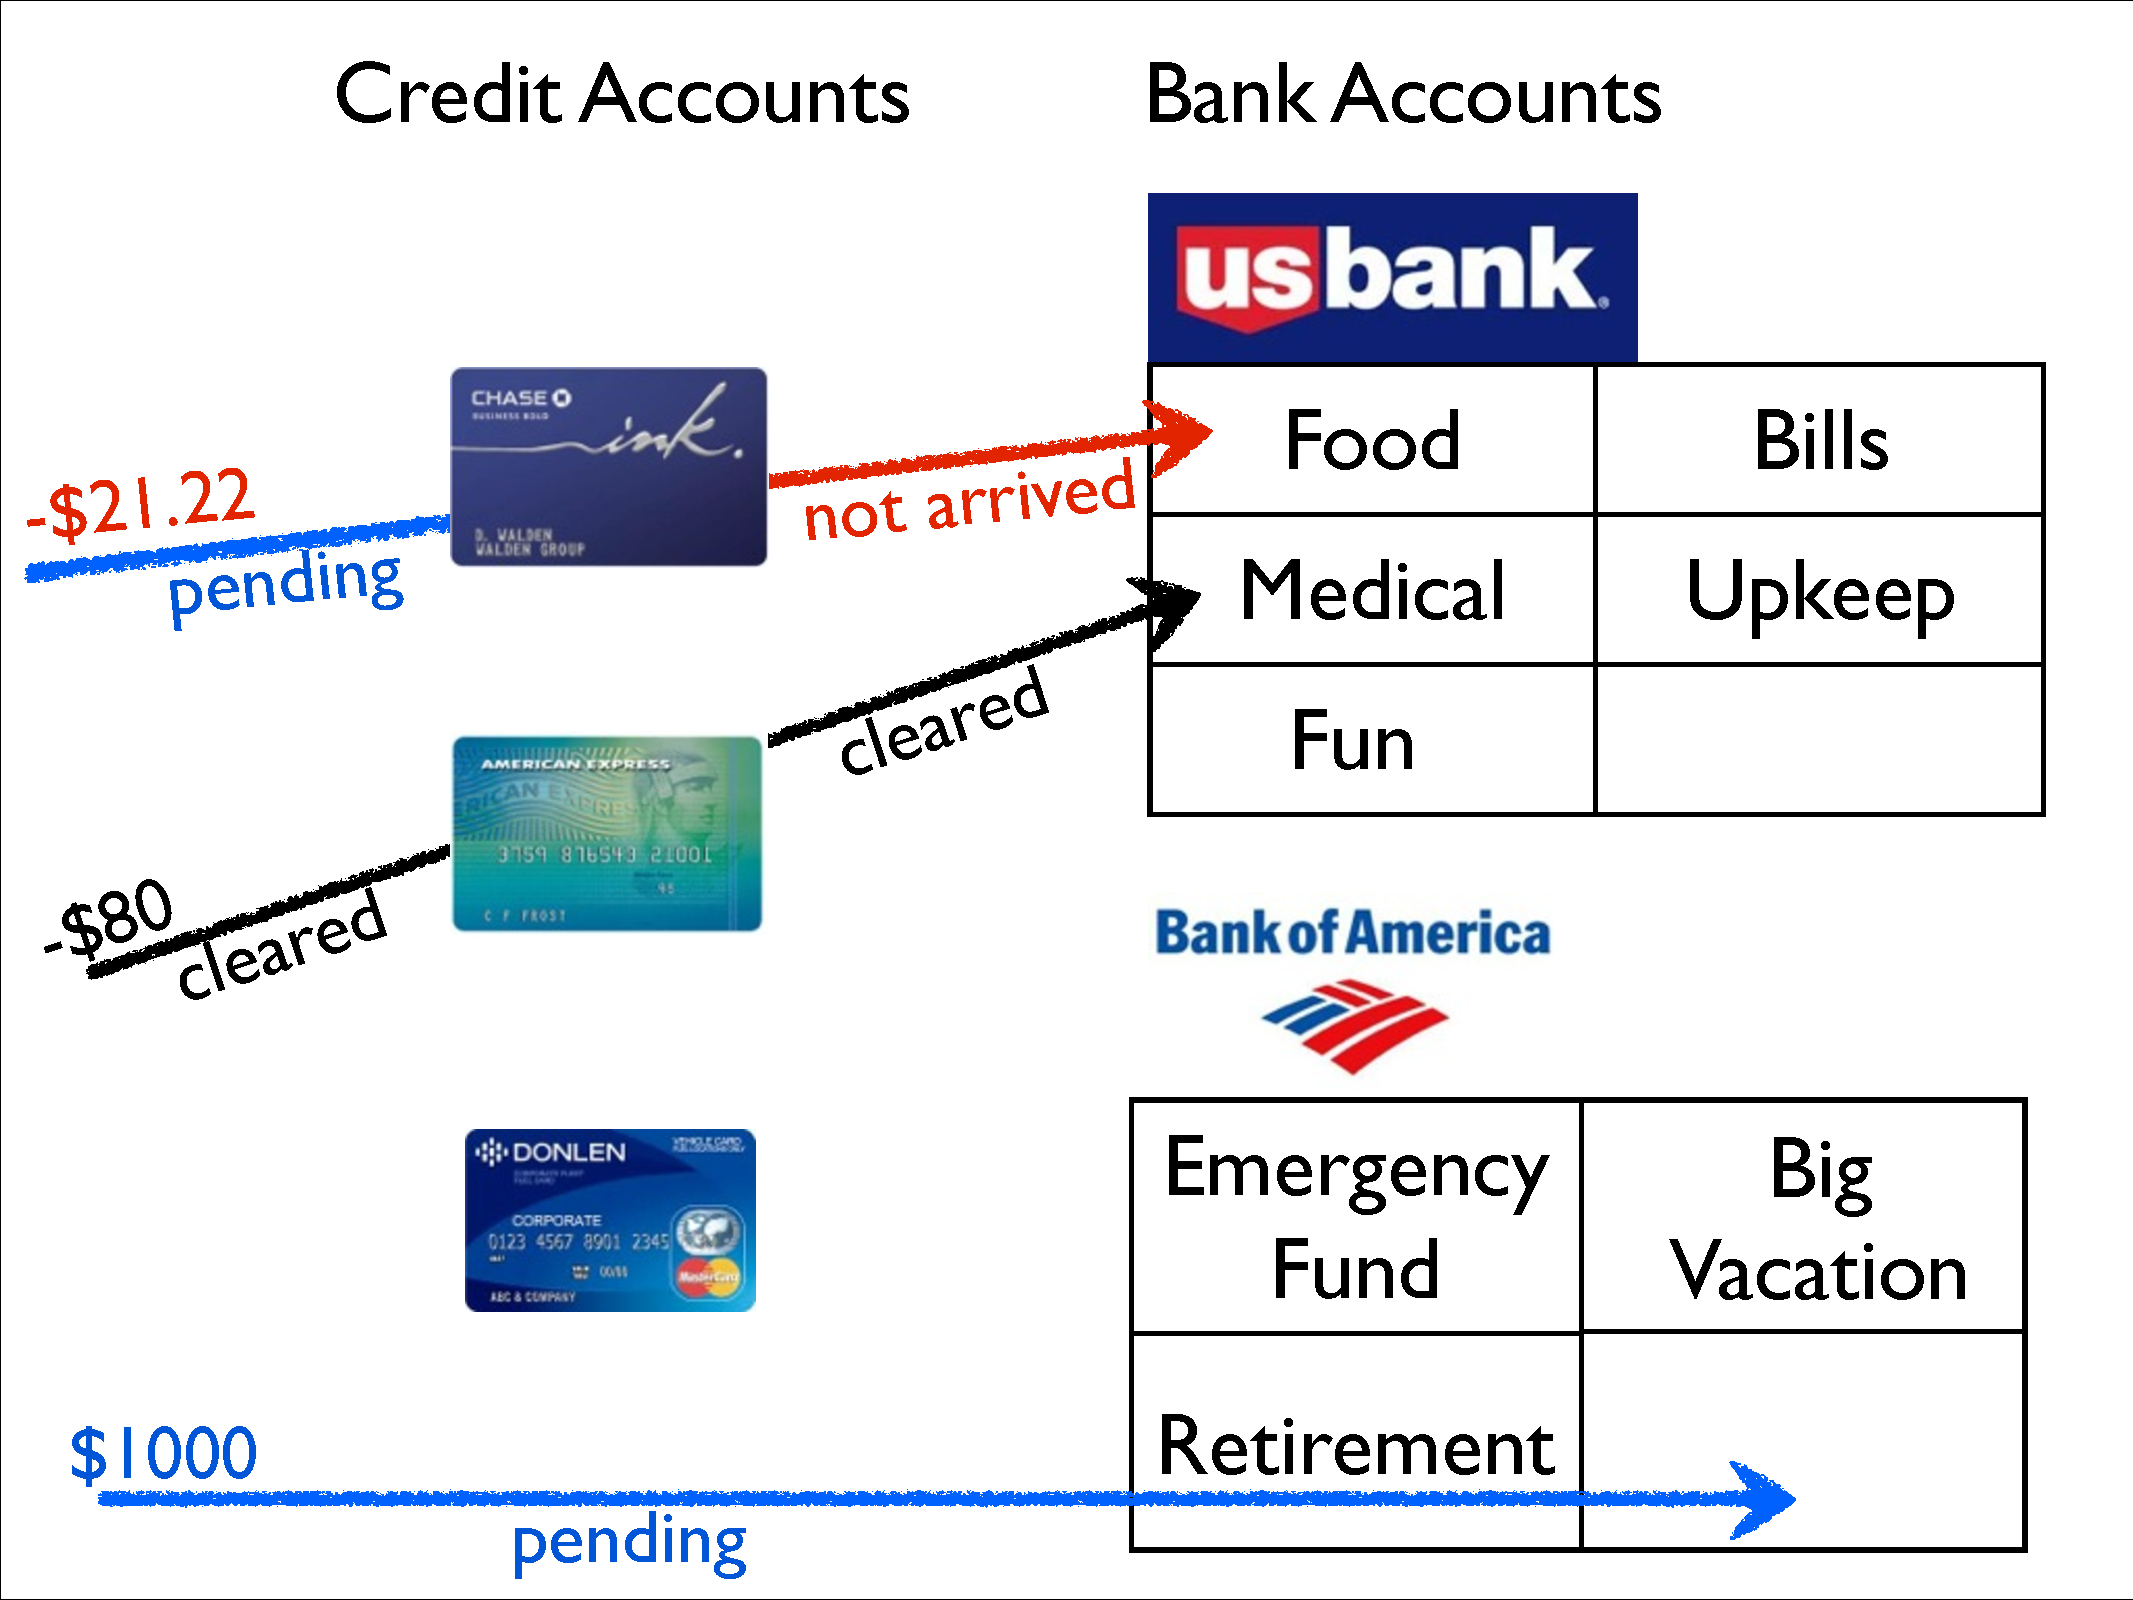
\includegraphics[scale=.4]{fig/model}
\end{center}

The amount, delay status, credit account, and bank account of each transaction are recorded in a tab-delimited file. For example, 

\begin{lstlisting}[language=bash, title=example\_ledger1.txt]
amount   status   credit        bank         partition   description
-21.22   cp       chase ink     us bank      food        groceries 12/7/13
-80               am ex         us bank      medical     coinsurance 
1000              bank of am                             misc savings
\end{lstlisting}  \q

Note that ``cp" in the status column indicates a transaction that is pending with respect to its credit account and still completely absent from its final destination bank account. For more information on transaction status codes, please see Section \ref{sec:codes}. 

\paragraph{} To output a summary of {\tt example\_ledger1.txt} on a Mac, I first locate and open Terminal. \q

\begin{center}
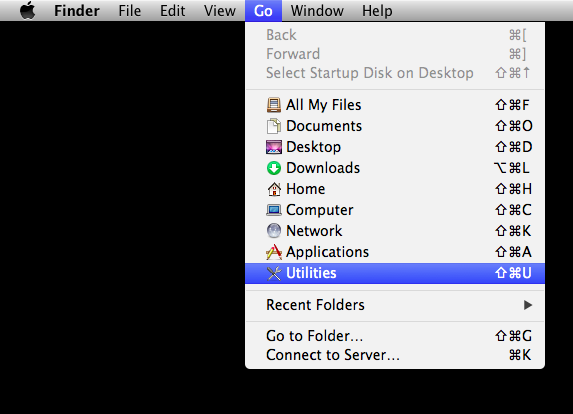
\includegraphics[scale=.75]{fig/open2.png}
\end{center} \q

\begin{center}
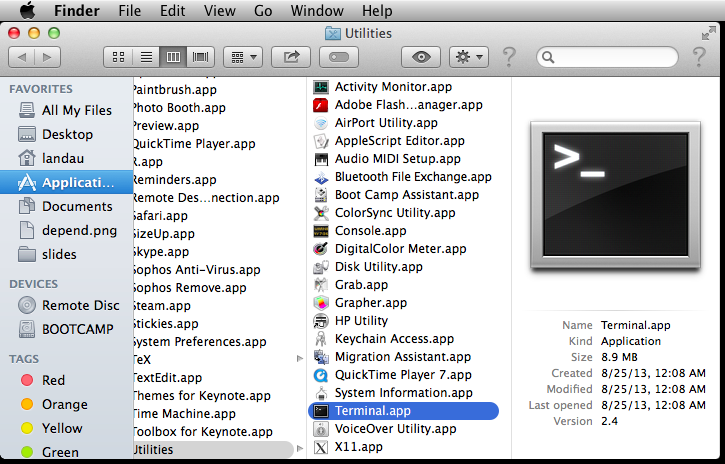
\includegraphics[scale=.6]{fig/open1.png}
\end{center} \q

Then, I compile and run the program in a Terminal window. \q

\begin{center}
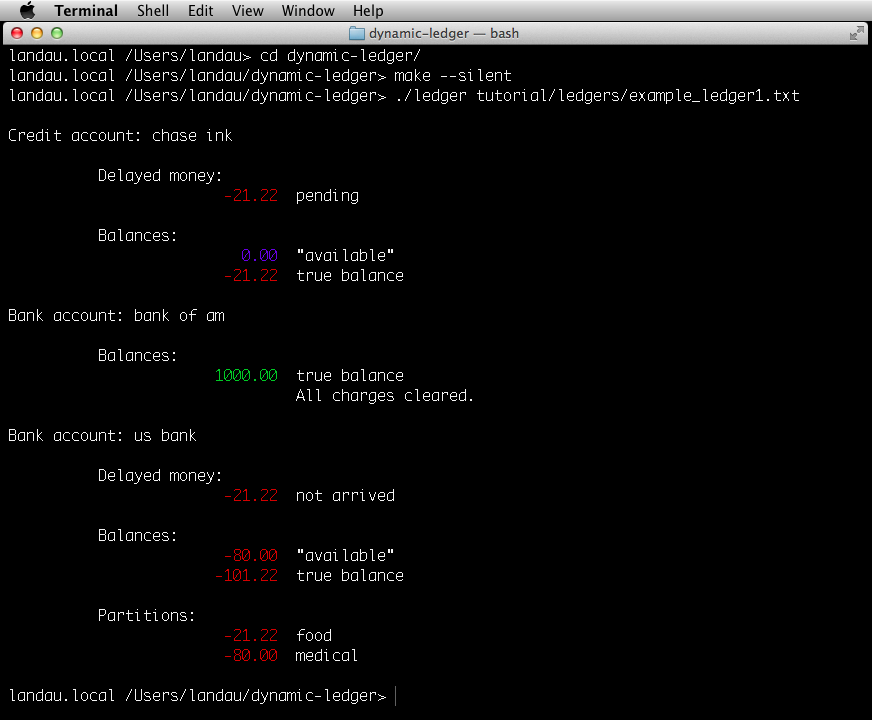
\includegraphics[scale=.5]{fig/open3.png}
\end{center} \q

The output gives the true balance of each account, along with other summaries that reflect transaction delays. Note that the program ignores accounts and partitions with balances of zero. 


\paragraph{} For the next major feature of the program, consider a longer ledger file.

\begin{lstlisting}[language=bash, title = example\_ledger2.txt]
amount   status   credit   bank       partition   description
-30.14   cn       card1    checking   food        groceries 12/3/13
-15.36   cn       card2    checking   food        produce 12/2/13
-10.41   cp       card1    checking   food        dinner 11/21/13
-7.31    c        card2    checking   fun         movie 11/18/13
-500     p                 checking   bills       December rent
-30      l                 checking   bills       November electric
-50      l                 checking   bills       November heat
-45                        checking   bills       The Economist
800      p                 checking   rent        November paycheck		
400      p                 checking   food        November paycheck	
500      p                 checking   upkeep      November paycheck		
50       p                 checking   fun         November paycheck	
50                         checking   fun         won $50 in poker		
200                        savings    bike        gift money
200                        savings    bike        October paycheck
100                        savings                general savings
200                                               cash
\end{lstlisting}  \q

The summary output for this file looks like

\begin{center}
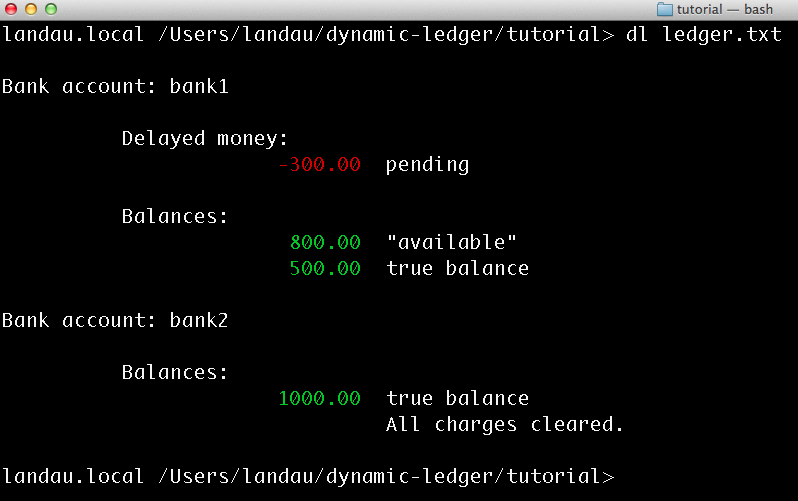
\includegraphics[scale=.5]{fig/sum1.png}
\end{center} \q



I may wish make a shorter ledger by condensing all the ``unlocked" (status $\ne$ ``l") transactions that have cleared.  In that case, I can simply run the program, but specify an output file. \q


\begin{center}
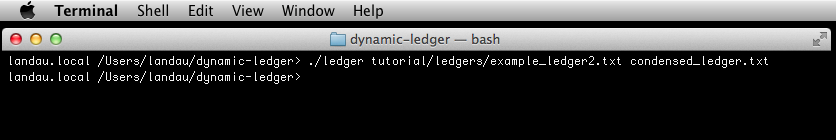
\includegraphics[scale=.5]{fig/condense.png}
\end{center} \q

The output, {\tt condensed\_ledger.txt}, contains only the locked transactions, delayed transactions, and bank partition totals. \q

\begin{lstlisting}[title=condensed\_ledger.txt]
amount    status	credit     bank        partition    description
-30.14    cn	    card1      checking    food         groceries 12/3/13
-15.36    cn	    card2      checking    food         produce 12/2/13
-10.41    cp      card1      checking    food         dinner 11/21/13
-7.31     c       card2      checking    fun          movie 11/18/13
-500.00   p                  checking    bills        December rent
-30.00    l	                 checking    bills        November electric
-50.00    l	                 checking    bills        November heat
800.00    p                  checking    rent         November paycheck
400.00    p                  checking    food         November paycheck
500.00    p                  checking    upkeep       November paycheck
50.00     p                  checking    fun          November paycheck
-45.00                       checking	   bills        condensed
50.00                        checking    fun          condensed
400.00                       savings     bike         condensed
100.00                       savings                  condensed
200.00                                                condensed
\end{lstlisting} \q

The summary output of {\tt condensed\_ledger.txt} agrees with that of  {\tt example\_ledger2.txt}.

\begin{center}
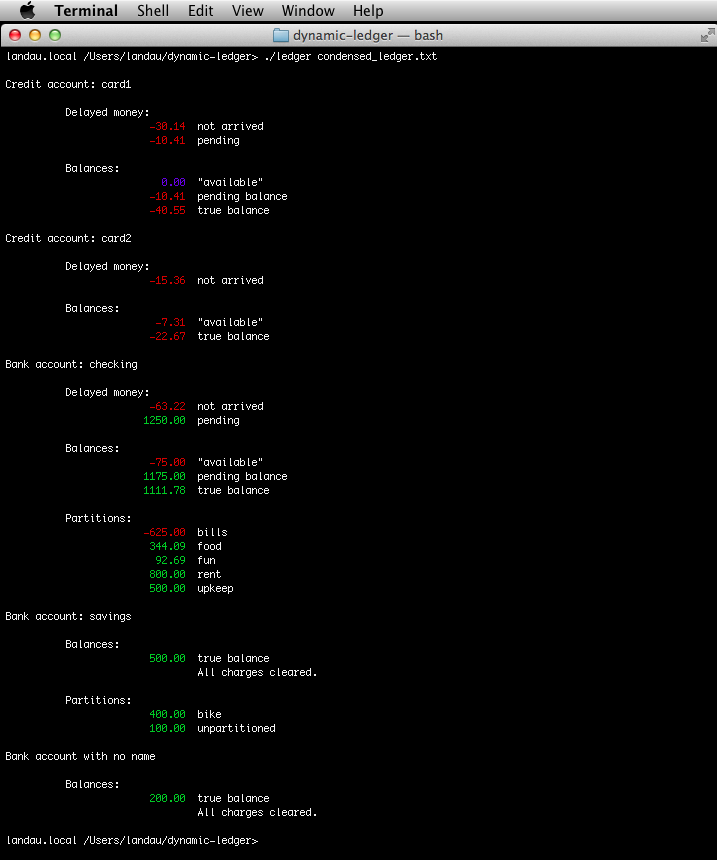
\includegraphics[scale=.5]{fig/sum2.png}
\end{center} \q



\section{Installation requirements}

\begin{itemize}
\item A command line interface program like Terminal. Windows users will need to download \href{http://www.cygwin.org}{Cygwin} or \href{http://www.mingw.org/}{MinGW}. (Command Prompt is not sufficient.)
\item The \href{http://gcc.gnu.org/}{GNU Compiler Collection}. Mac users should obtain it by installing \href{http://railsapps.github.io/xcode-command-line-tools.html}{Xcode command line tools}. Windows users should be able to obtain it through Cygwin or MinGW.
\end{itemize}


\section{Data format}

\paragraph{} Roughly speaking, each row in a ledger file represents a transaction, and each column represents a feature of that transaction. Here are more details about the columns.

\begin{center}
\begin{tabular}{lp{11cm}}
 {\tt amount} & Amount of money transferred in the transaction. All entries must be legal numbers. Negative numbers represent payments, and positive numbers represent deposits. \\ \\

{\tt status} & Transaction status codes, explained later, reflect the delay status of each transaction. A blank status indicates that the transaction has cleared. You can also use the status column to label any cleared transactions that you want to remain untouched in a condensed ledger. Warning: all unrecognized status codes will be ignored and those transactions will be treated as cleared. \\ \\

{\tt credit} & Names of the credit accounts. \\ \\

{\tt bank} & Names of the bank accounts. \\ \\

{\tt partition} & Names of the bank account partitions. It is useful to divide your accounts into different partitions: for example, food, medical, rent, etc. \\ \\

{\tt description} & A short memo describing the transaction, possibly including the merchant and the date. This field is the most flexible and it will not be processed by the program.
 
\end{tabular}
\end{center}

\section{Transaction status codes} \label{sec:codes}

\paragraph{} Transaction status codes are listed in the ``status" column of a ledger file, and they reflect the delay status of transactions. They are defined in {\tt include/user\_settings.h}. \q

\begin{lstlisting}
#define CREDIT_NOT_THERE_YET "cn" /*** HASN'T REACHED CREDIT COMPANY YET ***/
#define CREDIT_PENDING       "cp" /*** PENDING CHARGE IN CREDIT ACCOUNT ****/
#define CREDIT_CLEARED       "c"  /*** CLEARED IN CREDIT ACCOUNT ***********/
#define NOT_THERE_YET        "n"  /*** HASN'T REACHED BANK YET *************/
#define PENDING              "p"  /*** PENDING IN BANK *********************/
#define LOCKED               "l"  /*** CLEARED, BUT NOT OKAY TO CONDENSE ***/
\end{lstlisting} \q

Here is how you should think about transaction status codes. \q

\begin{center}
\begin{tabular}{lp{11cm}}
 {\tt CREDIT\_NOT\_THERE\_YET} & Say you just made a purchase with a credit card, but the transaction has not appeared yet on your credit company's website yet. Temporarily label transactions like these as such until the credit company thinks  that transaction is``pending"  or cleared . \\ \\

{\tt CREDIT\_PENDING} & Transactions shown as ``pending" in your account on your credit company's website. \\ \\

{\tt NOT\_THERE\_YET} & Say you wrote a check to a friend, but he's lazy and doesn't deposit it for two weeks. Transactions like these, which you know you made but do not appear on the webpage of your bank account yet, should be labeled as such. \\ \\

PENDING & Formally listed as ``pending" on your bank account website. \\ \\

LOCKED & Say you want to condense your ledger, but you do not want to lose the information for a particular transaction or set of transactions. Label these transactions as locked.
 
\end{tabular}
\end{center}



\section{Row and column separators}

\paragraph{} By default, the program expects the ledger file to have tab-delimited columns and rows delimited by either the newline character or the carriage return character. The user can change these settings at  \q

\begin{lstlisting}
#define ROW_SEPARATORS      "\n\r"
#define COLUMN_SEPARATORS   "\t" 
\end{lstlisting} \q

For example, If I change {\tt COLUMN\_SEPARATORS} to the comma, \q

\begin{lstlisting}
#define ROW_SEPARATORS      "\n\r"
#define COLUMN_SEPARATORS   "," 
\end{lstlisting} \q

then the program would expect a CSV (comma-separated values) file as input. These characters should only be used to separate fields. They should not be used in the actual entries of the ledger as content.



\section{Column order}


\paragraph{} The ordering of the columns in the ledger file is defined in the section of {\tt include/user\_settings.h} below.

\begin{lstlisting}
#define AMOUNT        0   /*** COLUMN FOR TRANSACTION AMOUNTS ************/
#define STATUS        1   /*** COLUMN FOR TRANSACTION STATUS CODES *******/
#define CREDIT        2   /*** COLUMN FOR NAMES OF CREDIT ACCOUNTS *******/
#define BANK          3   /*** COLUMN FOR NAMES OF BANK ACCOUNTS *********/       
#define PARTITION     4   /*** COLUMN FOR NAMES OF BANK PARTITIONS *******/
#define DESCRIPTION   5   /*** COLUMN FOR DESCRIPTIONS OF TRANSACTIONS ***/
\end{lstlisting} \q

The program would then expect a ledger file of the following form: \q

\begin{lstlisting}[language=bash]
amount   status   credit   bank       partition   description
-30.14   cn       card1    checking   food        groceries 12/3/13
-15.36   cn       card2    checking   food        produce 12/2/13
-10.41   cp       card1    checking   food        dinner 11/21/13
-7.31    c        card2    checking   fun         movie 11/18/13
-500     p                 checking   bills       December rent
-30      l                 checking   bills       November electric
-50      l                 checking   bills       November heat
-45                        checking   bills       The Economist
800      p                 checking   rent        November paycheck		
400      p                 checking   food        November paycheck	
500      p                 checking   upkeep      November paycheck		
50       p                 checking   fun         November paycheck	
50                         checking   fun         won $50 in poker		
200                        savings    bike        gift money
200                        savings    bike        October paycheck
100                        savings                general savings
200                                                  cash
\end{lstlisting} \q

which is the current default. But if I were to switch the order of the values of STATUS and AMOUNT, 

\begin{lstlisting}
#define AMOUNT        1   /*** COLUMN FOR TRANSACTION AMOUNTS ************/
#define STATUS        0   /*** COLUMN FOR TRANSACTION STATUS CODES *******/
#define CREDIT        2   /*** COLUMN FOR NAMES OF CREDIT ACCOUNTS *******/
#define BANK          3   /*** COLUMN FOR NAMES OF BANK ACCOUNTS *********/       
#define PARTITION     4   /*** COLUMN FOR NAMES OF BANK PARTITIONS *******/
#define DESCRIPTION   5   /*** COLUMN FOR DESCRIPTIONS OF TRANSACTIONS ***/
\end{lstlisting} 

\q 
Then the program would expect a ledger file of the form,\q

\begin{lstlisting}[language=bash]
status   amount   credit   bank       partition   description
cn       -30.14   card1    checking   food        groceries 12/3/13
cn       -15.36   card2    checking   food        produce 12/2/13
cp       -10.41   card1    checking   food        dinner 11/21/13
c        -7.31    card2    checking   fun         movie 11/18/13
         -500              checking   bills       December rent
l        -30               checking   bills       November electric
l        -50               checking   bills       November heat
         -45               checking   bills       The Economist
p        800               checking   rent        November paycheck		
p        400               checking   food        November paycheck	
p        500               checking   upkeep      November paycheck		
p        50                checking   fun         November paycheck	
         50                checking   fun         won $50 in poker		
         200               savings    bike        gift money
         200               savings    bike        October paycheck
         100               savings                general savings
         200                                      cash
\end{lstlisting}




\section{Summary output options}

\paragraph{} The user can tweak some of the macros in {\tt user\_settings.h} to customize the output of the summaries.

\begin{lstlisting}
#define PRINT_ZEROED_ACCOUNTS   0

#define USE_COLOR    1

#define NORMAL_COLOR     "\x1B[0m"    /*** REGULAR TEXT ******/
#define NEGATIVE_COLOR   "\x1B[31m"   /*** NEGATIVE TOTALS ***/
#define POSITIVE_COLOR   "\x1B[32m"   /*** POSITIVE TOTALS ***/
#define ZERO_COLOR       "\x1B[34m"   /*** EMPTY TOTALS ******/
\end{lstlisting}


\begin{center}
\begin{tabular}{lp{11cm}}
{\tt PRINT\_ZEROED\_ACCOUNTS} & Set to 1 to print out all accounts, including those with balances of \$0.00. Set to 0 to ignore all empty accounts. \\ \\

{\tt USE\_COLOR} & Set to 1 to print out summaries in color. Set to 0 otherwise. Coloring is best for viewing summaries
in the terminal window, but if you want to pipe the output to a file and view it there, then the color codes create extra 
annoying characters. \\ \\

{\tt NORMAL\_COLOR } & Shell color code for regular text. The default is white. \\ \\

{\tt POSITIVE\_COLOR } & Shell color code for positive totals in the summaries. The current default is green. \\ \\

{\tt NEGATIVE\_COLOR } & Shell color code for negative totals. The current default is red. \\ \\

{\tt ZERO\_COLOR } & Shell color code for zero totals. The current default is blue. \\ \\


\end{tabular}
\end{center}



\section{Disclaimer}

\paragraph{} This software is still new and may still have nontrivial bugs. Also, I have not actually implemented some of the minor features I described here. In particular, some of the user settings are not supported yet.


\section{License}

\paragraph{} This software is licensed under the GNU public license 3.0. 





\end{flushleft}
%\newpage 
%\bibliographystyle{plainnat} 
%\bibliography{}
\end{document}